%\graphicspath{{/media/data/Work/cnstellate/DS_ClickRecovery/}{/media/data/Work/Responses/}{../figures/}{./gfx/}}
%===================================
\section[DS Cell Model]{D~Stellate Cell Model: Optimisation using click recovery responses}   \label{sec:d-stellate-cell-model}

\subsection{Introduction}

This section shows the GABAergic input and intrinsic cell properties influence the behaviour of D~stellate cells.
In the mammalian \CN, the \VCN~\DS cells~have a wide ranging influence on almost all primary cells of the \CN\@.  
Glycinergic terminals of the DS cell contact T~stellate and bushy neurons in the \VCN \citep{RhodeSmithEtAl:1983}, fusiform and tuberculoventral cells in the the ipsilateral \DCN~(type II and type IV \EIRA~units), and some DS cells are commissural the contralateral \CN~\citep{NeedhamPaolini:2007}.

% \smallskip{}

% Large multipolar or stellate cells in the \VCN~have been shown to have 3--4
% long dendrites stretching 200 microns (or one third of the \VCN) and their
% axonal collaterals cover the same region in the \VCN, almost one half of the
% \DCN, and are one source of the commissural projection to the contralateral
% cochlear nucleus \citep{NeedhamPaolini:2007}.
%%%%%%%%%%%%%%%%%%% Copied from original jneurometh article

\DS~cells are large multipolar neurons in the \VCN~and have an \OnC~\PSTH~to tones and noise \citep{SmithRhode:1989,NeedhamPaolini:2006}.
They typically have 3--4 long dendrites stretching 200 microns (or one third of the \VCN) and their axonal collaterals cover the same region in the \VCN, almost one half of the \DCN, and are one source of the commissural projection to the contralateral cochlear nucleus \citep{Cant:1992,Cant:1981,SchofieldCant:1996,CantBenson:2003,NeedhamPaolini:2007,PaoliniClark:1999}.
Intracellular responses to sounds indicate the bandwidth of inputs to \DS~neurons typically ranges from two octaves below \CF~to one octave above \CF~\citep{PalmerJiangEtAl:1996,JiangPalmerEtAl:1996,PaoliniClark:1999}.
\DS~cell axon terminals contain the inhibitory neurotransmitter glycine and synapse widely in the \VCN~and \DCN\.
They also send a commissural projection to the contralateral cochlear nucleus that mediates fast inhibition between the nuclei \citep{NeedhamPaolini:2003,NeedhamPaolini:2006,Oertel:1997}.

% \smallskip{}

Post-onset GABAergic inhibition in \DS~cells is a major influence on the \PSTH~of \OnC~neurons \citep{FerragamoGoldingEtAl:1998a,EvansZhao:1998}.
Latency of excitation to auditory nerve shocks suggests Golgi cells are activated by type II \ANFs~and low spontaneous rate type I~\ANFs~\citep{BensonBerglundEtAl:1996,FerragamoGoldingEtAl:1998}.
Therefore, type II and \LSR~type I \ANFs~could be involved in gain control through GABAergic modulation of activity in the \VCN.

% \smallskip{}

\GABA~blockers in the \VCN~have a significant effect of changing the behaviour in the response to AM in the IC \citep{CasparyPalombiEtAl:2002}.  AM coding effects of GABA in the Chinchilla
% \CN~\citep{BackoffShadduckEtAl:1999}. \citep{CasparyBackoffEtAl:1994} Caspary
% and colleagues worked on the effects of \GABA~in in the \VCN.

% Zhang and Winter looked at the response area of \VCN~onset units to determine
% \GABA~{on\slash off} freq.

% Smith and Rhode, Smith and others looked at OnC response area and two-tone

%===================================
\subsection{Implementation}


% 2.5. Data analysis
% Data were collected as spike times with a resolution of 10
% μs and analyzed off-line on a micro-VAX 3100 (Digital). Response histograms
% were plotted and analyzed using a windowing technique in which spike counts
% were taken over brief time windows of identical duration for the masker and
% probe components (Fig. 1B). Using the control conditions, counting windows
% were determined individually for each unit but ranged between 1 and 4 ms based
% on the control response to the masker alone and the probe alone. To assess
% response variability over time, repeated unmasked controls for both the masker
% (masker alone, Ma) and probe (probe alone, Pa) were obtained during the
% pre-drug, drug, and post-drug recovery conditions. Drug doses were determined
% empirically as the lowest dose that elicited a reproducible and reversible
% effect. To allow normalization of the masked probe response obtained in the
% paired-click paradigm to the unmasked response obtained when the probe was
% presented alone, identical measurement windows were used in the control and
% drug conditions for a given unit. The suppression recovery functions for each
% unit were normalized by taking the ratio Pm/Pa where Pm is the masked probe
% spike count and Pa is the unmasked response to the probe (Fig. 1C).



Key elements in the creation of the D~stellate cell model are shown in the Nordlie table~\ref{tab:DScellModelSummary}A.
A type I-II single compartment neuron by \citet{RothmanManis:2003b} has the characteristics of a onset chopper unit and has previously been used to simulate a \DS~cell model.
The choice of having a large multipolar neuron without dendrites was based on computational efficiency and ensuring that the model fit within the criteria for DS cells.
The electrotonic dendrites of \DS~cells mean that the filtering in \DS~cells primarily controls the height of excitatory {\PSPs} reaching the soma \citep{WhiteYoungEtAl:1994}, hence a single compartment with graded weights should suffice.


The synaptic connections onto the D~stellate cell model, shown in table~\ref{tab:DScellModelSummary}C, are simplified to afferent ANF inputs and intra-nuclear col-localised GABAergic input from Golgi cells.
The \ANF~spread onto \DS~cells is well documented \citep{PaoliniClark:1999,ArnottWallaceEtAl:2004,PalmerWallaceEtAl:2003,JiangPalmerEtAl:1996,PalmerJiangEtAl:1996}, hence a decision made to fix this parameter due to the large computational task of calculating an optimisation routine for \ANFDS bandwidth.
The spread \ANF~to \DS~cells (\sANFDSh,\sANFDSl) is set so that 2 octaves below and 1 octave above \CF~are within 2 standard deviations \citep{PaoliniClark:1999}.


The physiological effect of GABAergic inputs onto onset choppers is primarily on CF~\citep{CasparyHaveyEtAl:1979,PalombiCaspary:1992,CasparyBackoffEtAl:1994,CasparyPalombi:1993,CasparyPalombiEtAl:1993}, but the bandwidth is difficult to ascertain.
The dendrites of D~stellate cells cover one third of the nucleus (approximately 3 octaves of tonotopic frequencies) and occasionally project into the \GCD~\citep{ArnottWallaceEtAl:2004}.
Golgi cells' axonal collaterals are confined to 200 microns in the \GCD~and \ANF~tonotopic organisation in the \GCD~is less defined.
The \GLGDS~spread is set to 2 channels with zero offset, which corresponds to a \DS~cell selecting from approximately 5 nearest Golgi cells.

\begin{figure}[htb]
  \centering
%  \resizebox{0.8\textwidth}{!}{}
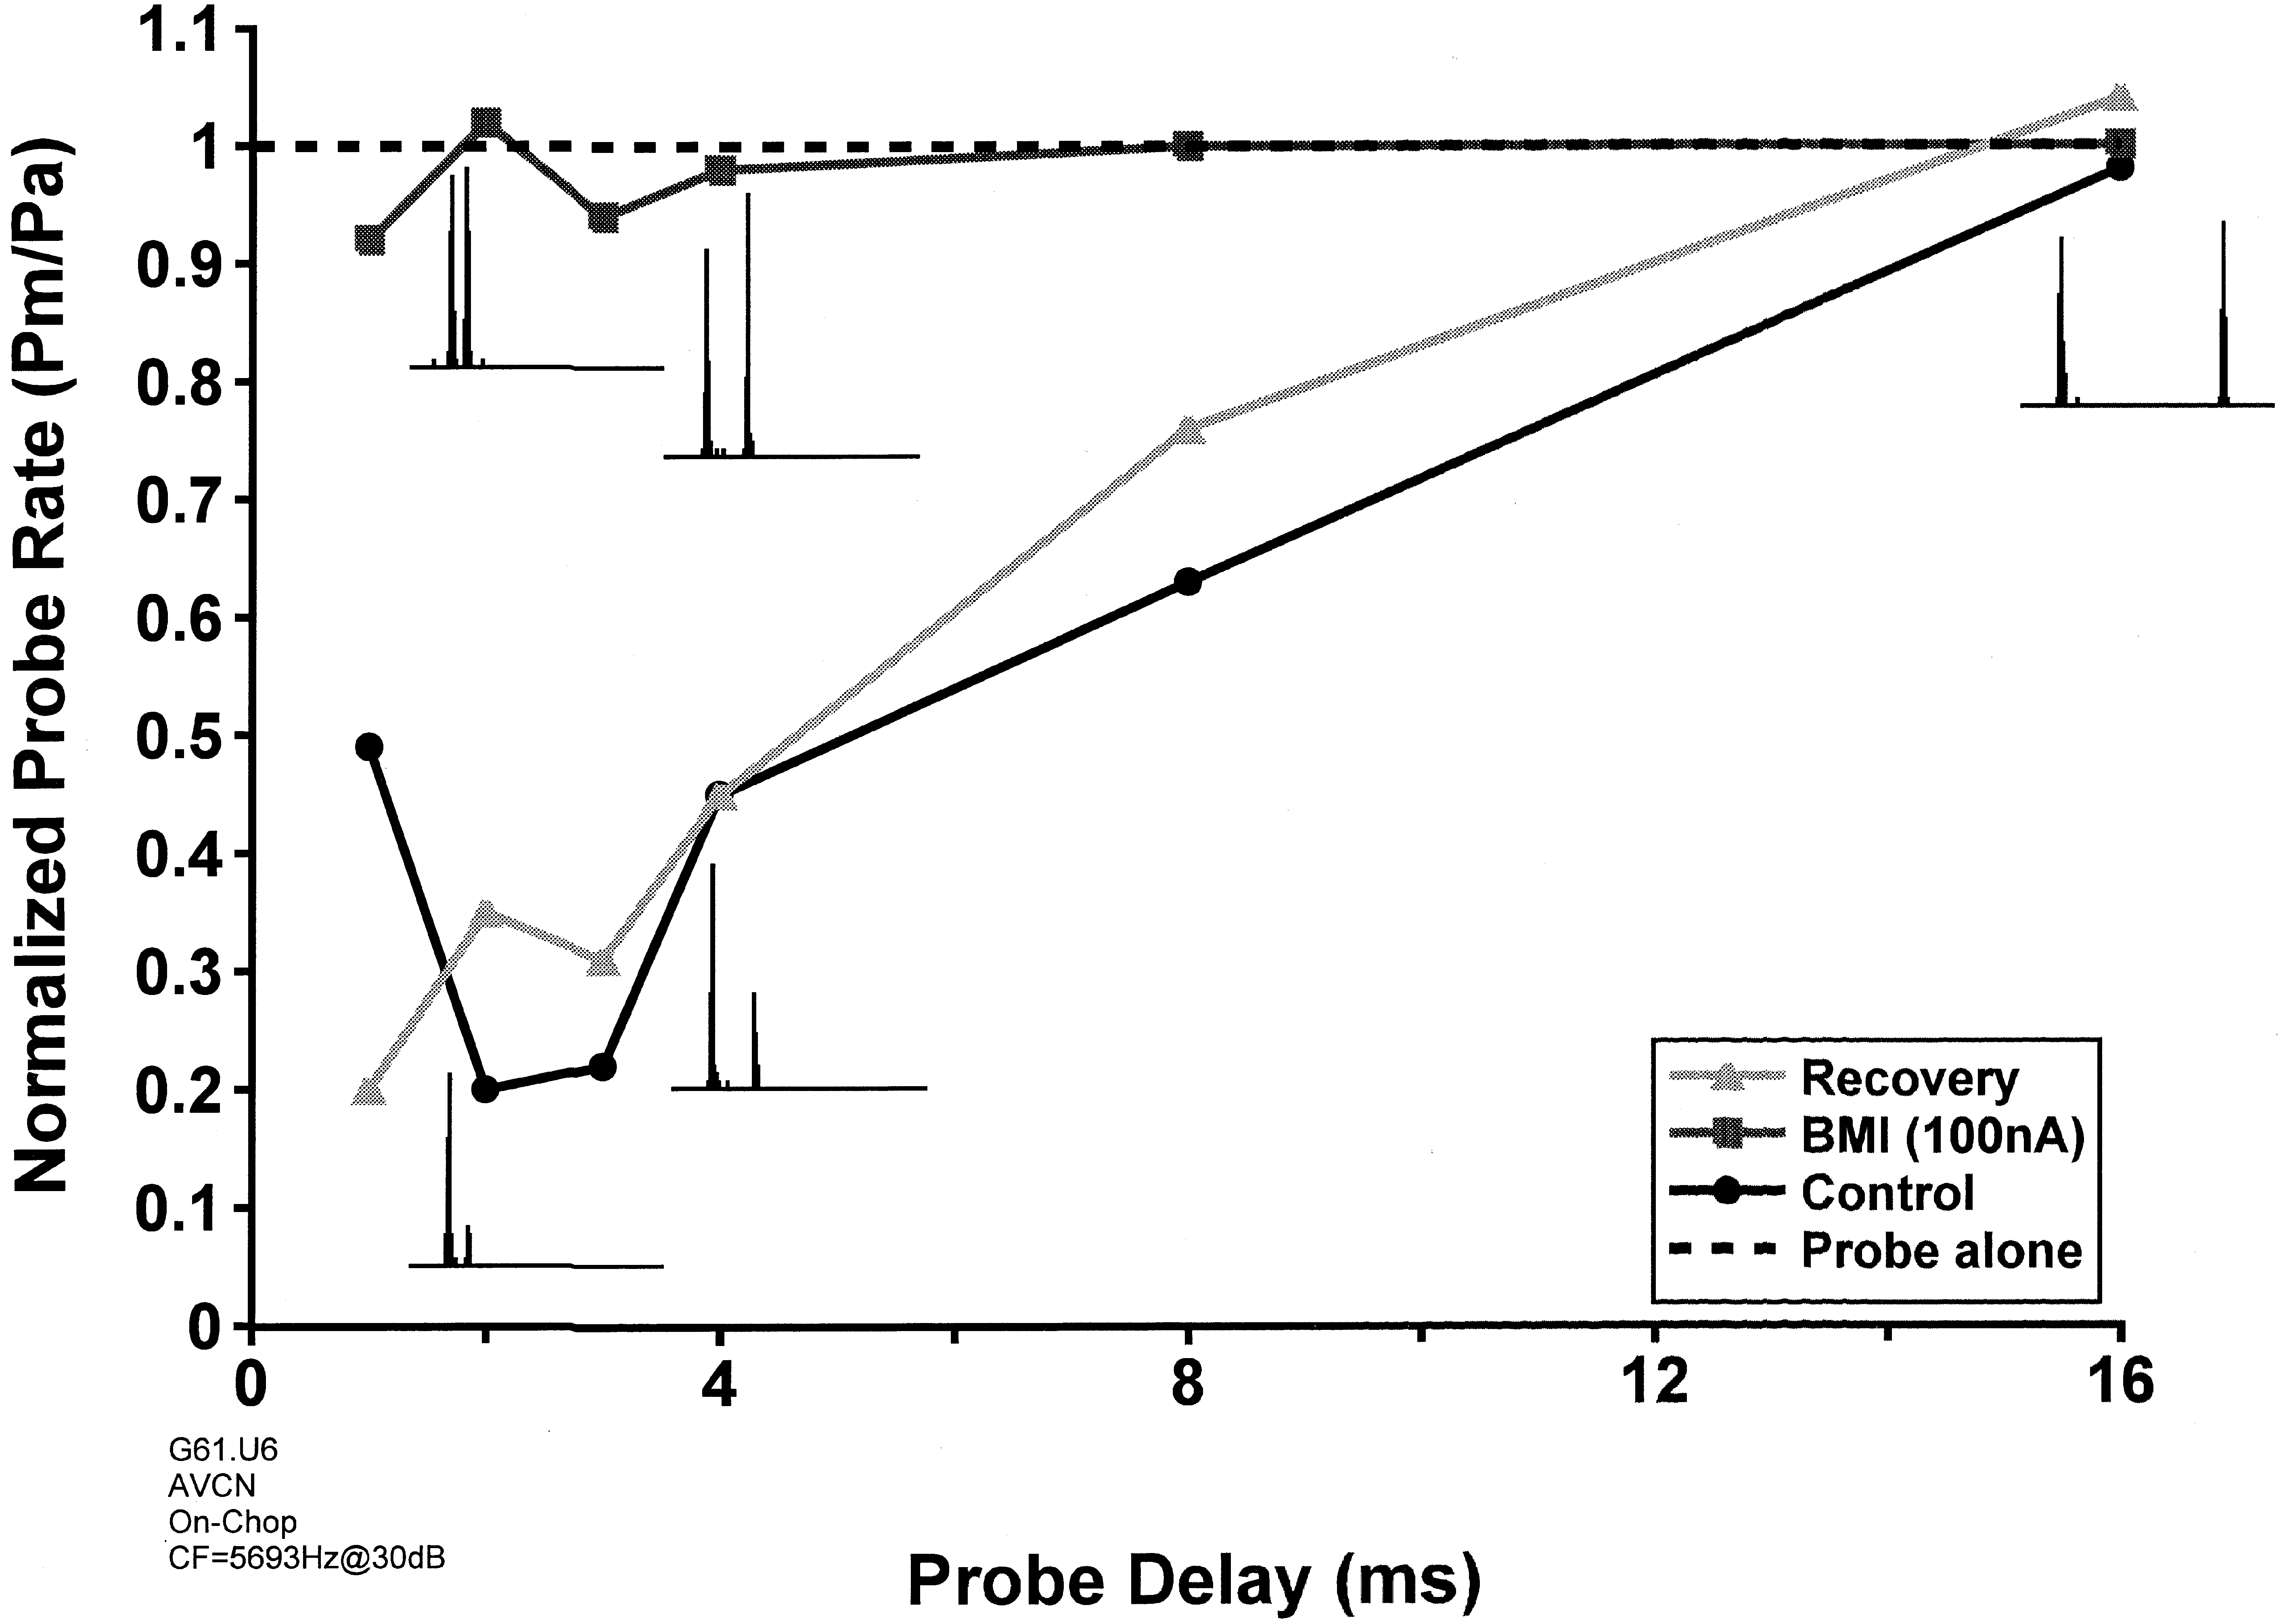
\includegraphics[keepaspectratio,width=0.8\textwidth]{gfx/Backoff+Palombi-Fig3}
\caption{Experimental data showing click recovery in onsetchoppers
\yellownote{Permission needed}
\label{fig:BackoffPalombi}}
\end{figure}

\DS input parameters that were preemptively fixed included: the number of \GLG to \DS synapses ($\nGLGDS = 25$), the spread of \ANFs~to \DS~cells (\sANFDSh and \sANFDSl), and the conduction delay from the auditory nerve (\dANFDS).
The first spike latency in high \CF \DS~cells ($2.8 \pm 0.09$ ms) is precise and faster than other stellate neurons in the VCN \citep{RhodeSmith:1986}.
The addition of 0.5~ms to \ANFDS~connections is a combination of conductance and synaptic delay.

%%The effect of Golgi cells on \DS~is delayed by the extra 0.7~ms delay from \ANF~to Golgi, plus the slow peak of \GABAa~inhibition.
%\yellownote{fix this paragraph}


%%% Local Variables:
%%% mode: latex
%%% mode: tex-fold
%%% mode: visual-line
%%% TeX-master: "SimpleResponses"
%%% TeX-PDF-mode: nil
%%% End:
